\section{Discussion}

Taking the XFoil data as "experimental," and the CFD data as numerical prediction, error bars of $\pm10\%$ were drawn from each XFoil data point. Observing the $C_l$ first in Fig. \ref{fig:error_bar1}, XFoil and CFD agree very well with the exception of AoA = -2 deg (I need to double check this run), where there is a noticeable deviation. This difference is unexpeced because all other predictions in this attached regime aligns quite well. Also, the AoA of separation is lower as predicted by CFD. In this case, the CFD simulation might be more trustworthy, as it is difficult to predict separation, especially with low-fidelity methods. Regarding $C_d$, the CFD generally overpredicted the XFoil solution as seen in Figs. \ref{fig:error_bar2} and \ref{fig:error_bar3}, zoomed-in view of the exact same same figure. The former is at small negative AoAs, where the CFD prediction is about 10\% above XFoil prediction; this was as close as the two solutions ever came. Higher AoAs led to larger discrepancies, where the CFD predictions increasingly overpredicted the XFoil estimates.

\begin{figure}[H]
\centering
    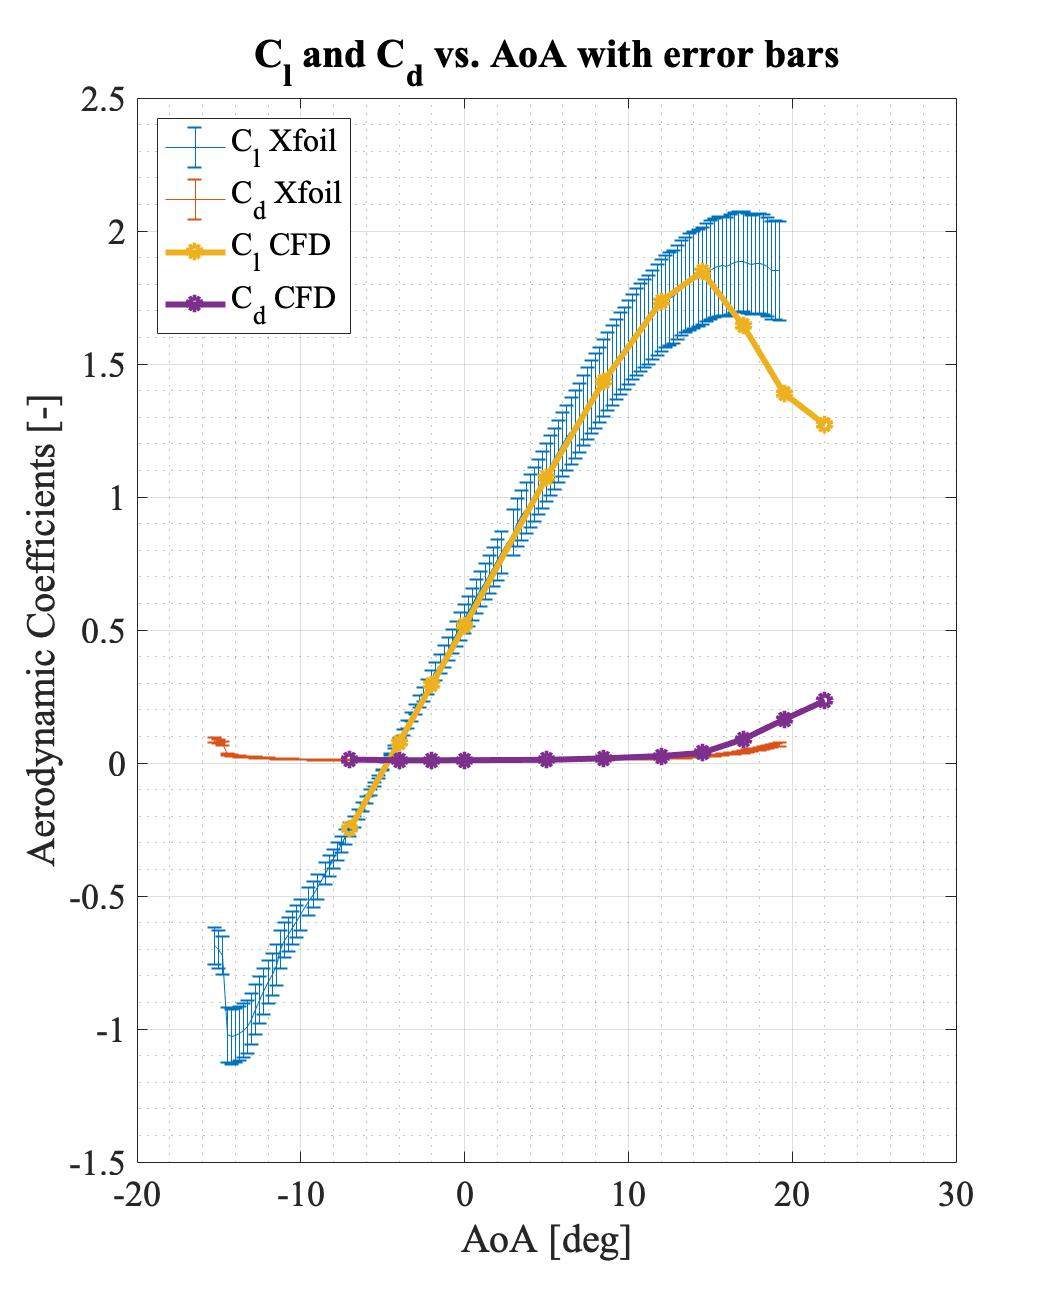
\includegraphics[width=0.65\textwidth]{error_bar1.jpg}
    \caption{$C_l$ and $C_d$ comparisons including error bar of $\pm$10\%}
    \label{fig:error_bar1}
\end{figure}

\begin{figure}[H]
  \begin{subfigure}[b]{0.5\textwidth}
    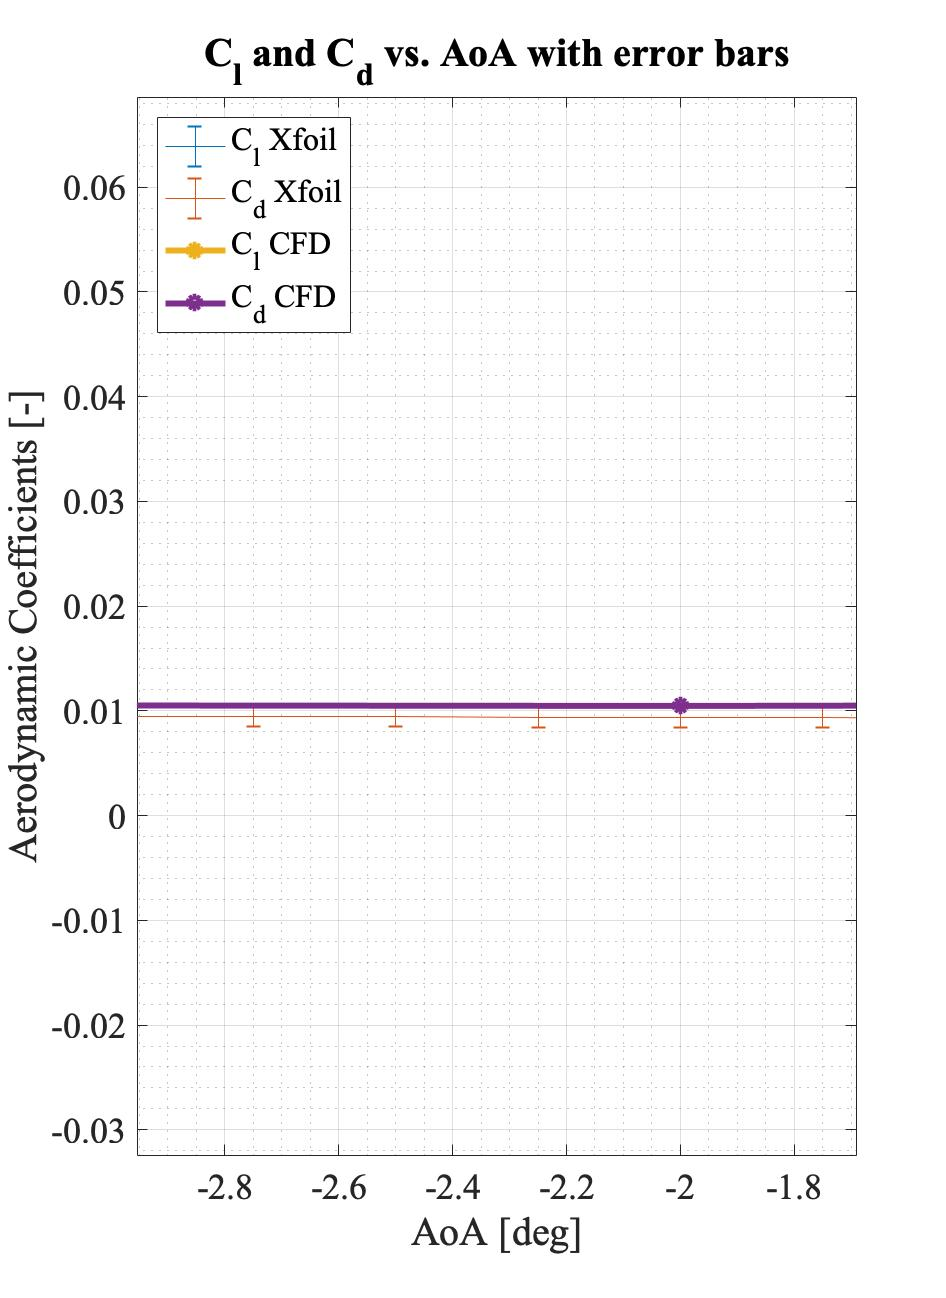
\includegraphics[width=\textwidth]{error_bar2.jpg}
    \caption{Zoomed-in view of lower AoA section of $C_d$}
    \label{fig:error_bar2}
  \end{subfigure}
  \begin{subfigure}[b]{0.5\textwidth}
    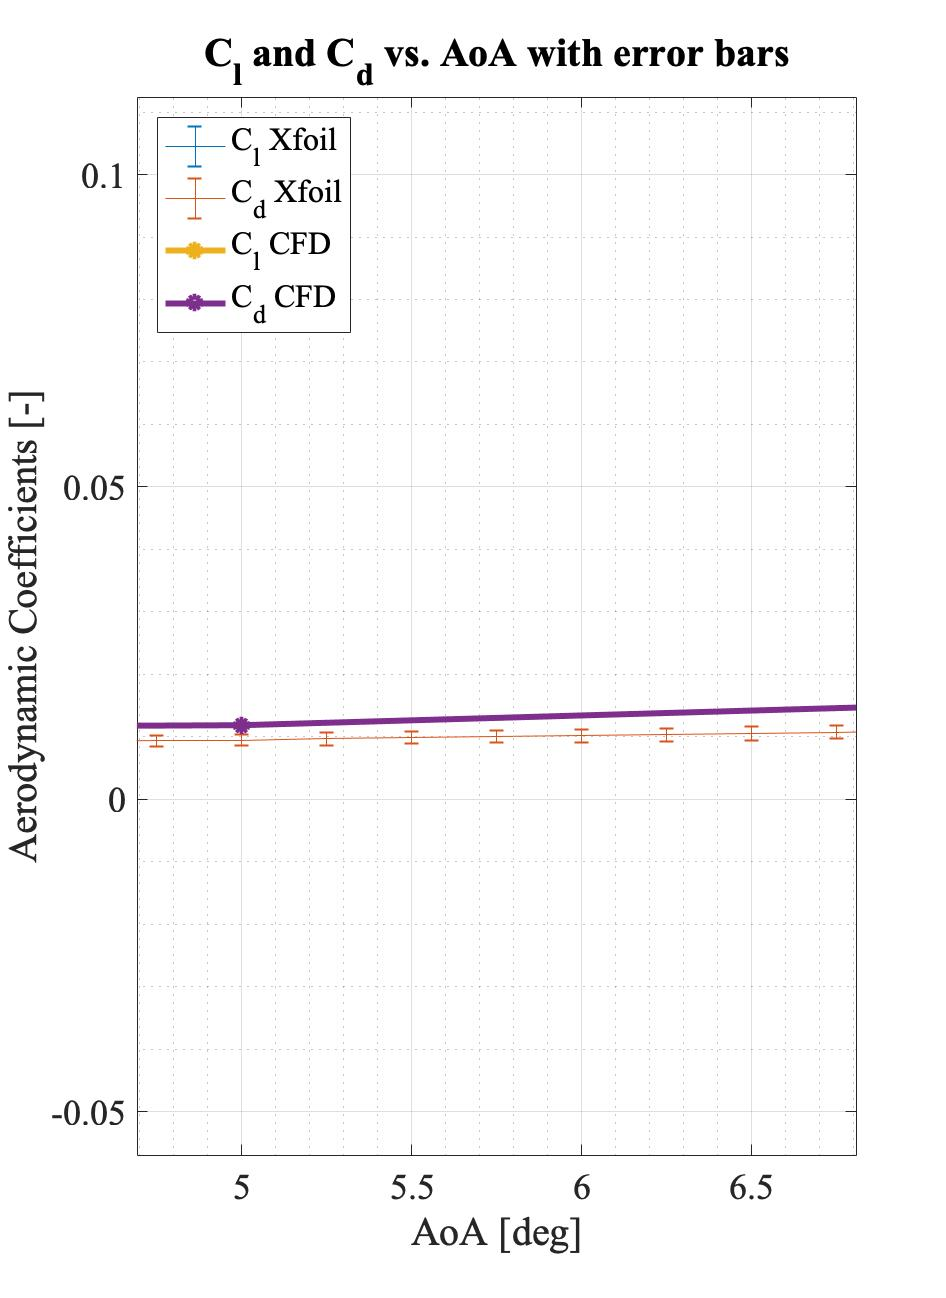
\includegraphics[width=\textwidth]{error_bar3.jpg}
    \caption{Another zoomed-in view of larger AoA section of $C_d$}
    \label{fig:error_bar3}
  \end{subfigure}
\end{figure}
